\section{Фреймворк DPDK}

Ввиду описанных в пункте 3.1 недостатков существующих систем сбора сетевого трафика, было принято решение разработать собственную систему сбора, удовлетворяющую следующим требованиям:
\begin{itemize}
\item достаточная для корректного сбора трафика скорость обработки пакетов;
\item потенциальная возможность анализа всего трафика в режиме реального времени;
\item соответствие и безболезненная интеграция в существующую сетевую инфраструктуру.
\end{itemize}

Таким образом, было решено разрабатывать систему сбора сетевого трафика, основанную на технологии DPDK.\par 

DPDK --- это фреймворк, который предоставляет набор библиотек и драйверов для ускорения обработки пакетов в приложениях, работающих на архитектуре Intel. DPDK поддерживается на любых процессорах Intel от Atom до Xeon, любой разрядности и без ограничения по количеству ядер и процессоров. В настоящее время DPDK портируется и на другие архитектуры, отличные от x86 --- IBM Power 8, ARM и др.\par 

DPDK позволяет полностью исключить сетевой стек Linux из обработки пакетов. Приложение, работающее в User Space, напрямую общается с аппаратным обеспечением.\par 

\begin{figure}[h!]
    \centering
    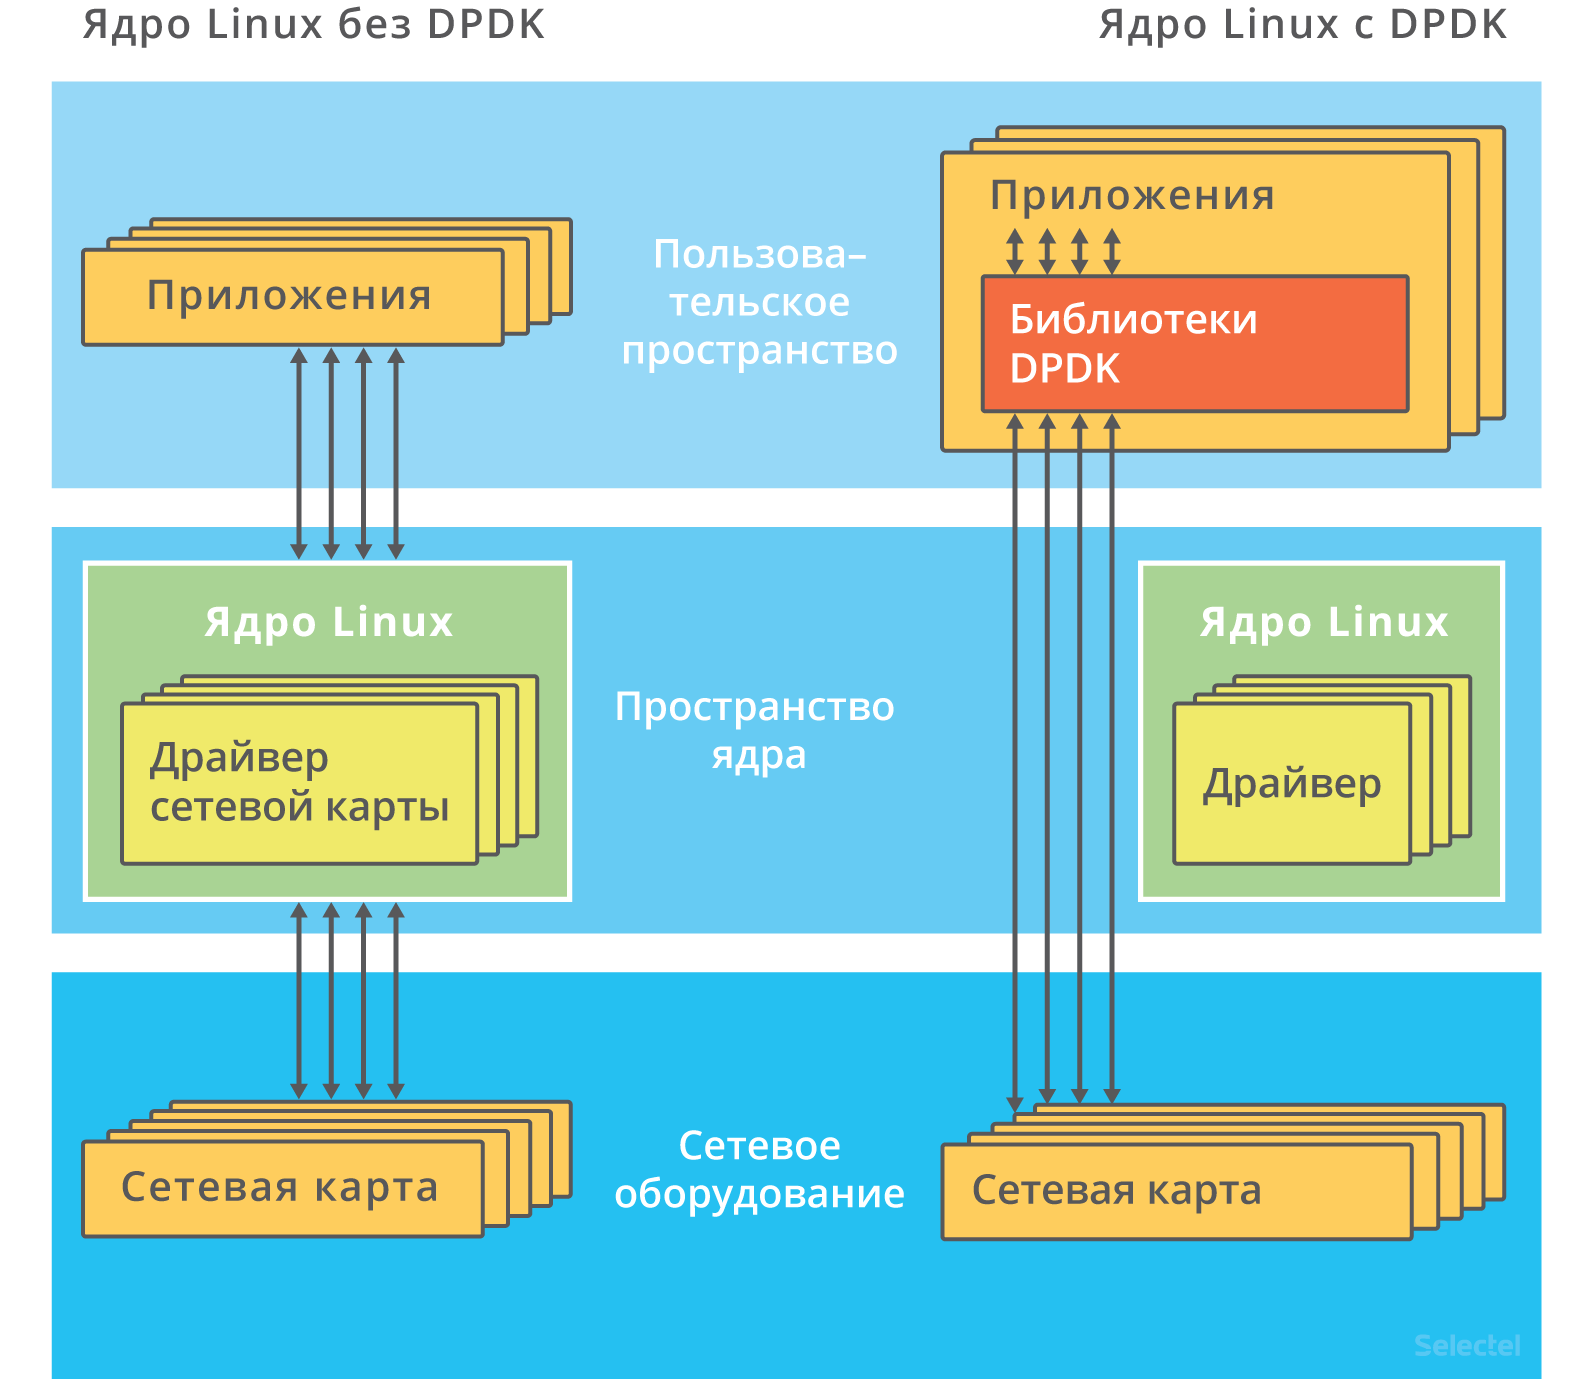
\includegraphics[width=0.7\textwidth]{5}
    \caption{Схема работы DPDK}
    \label{img:5}
\end{figure} 

Использование DPDK также позволяет привязывать задачу к определенному ядру. Это исключает накладные расходы, создаваемые планировщиком Linux при переключении задач. Благодаря использованию многопоточности, DPDK сокращает количество обращений к памяти и PCI, более эффективно используя процессорные мощности. Также DPDK позволяет оптимизировать использование памяти путем выравнивания структуры данных к размеру кэша, тем самым сводя к минимуму доступ к внешней памяти.\par

Наибольший прирост производительности можно увидеть при обработке большого количества маленьких пакетов. На графике ниже приведено сравнение производительности L3 forwarding c использованием DPDK и без него.\par 

\begin{figure}[h!]
    \centering
    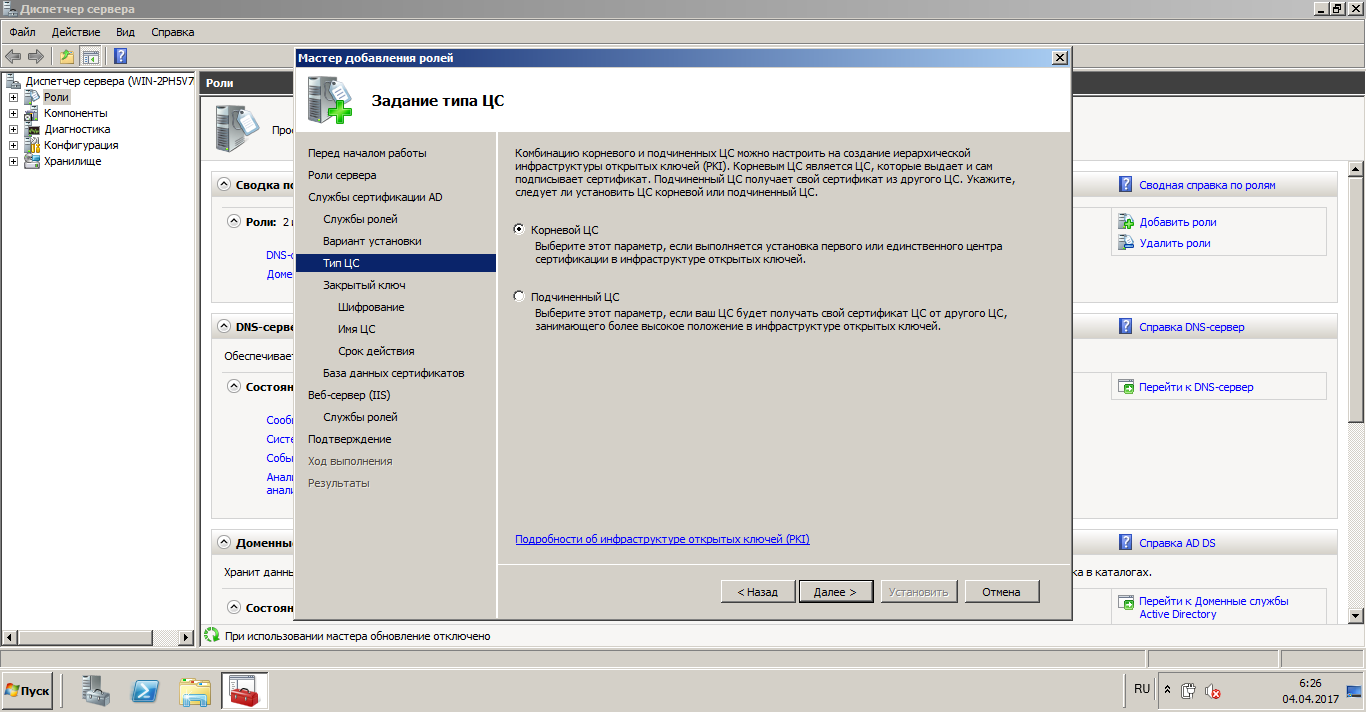
\includegraphics[width=0.7\textwidth]{6}
    \caption{Сравнение производительности L3 forwarding c использованием DPDK и без него}
    \label{img:6}
\end{figure} 

\begin{figure}[h!]
    \centering
    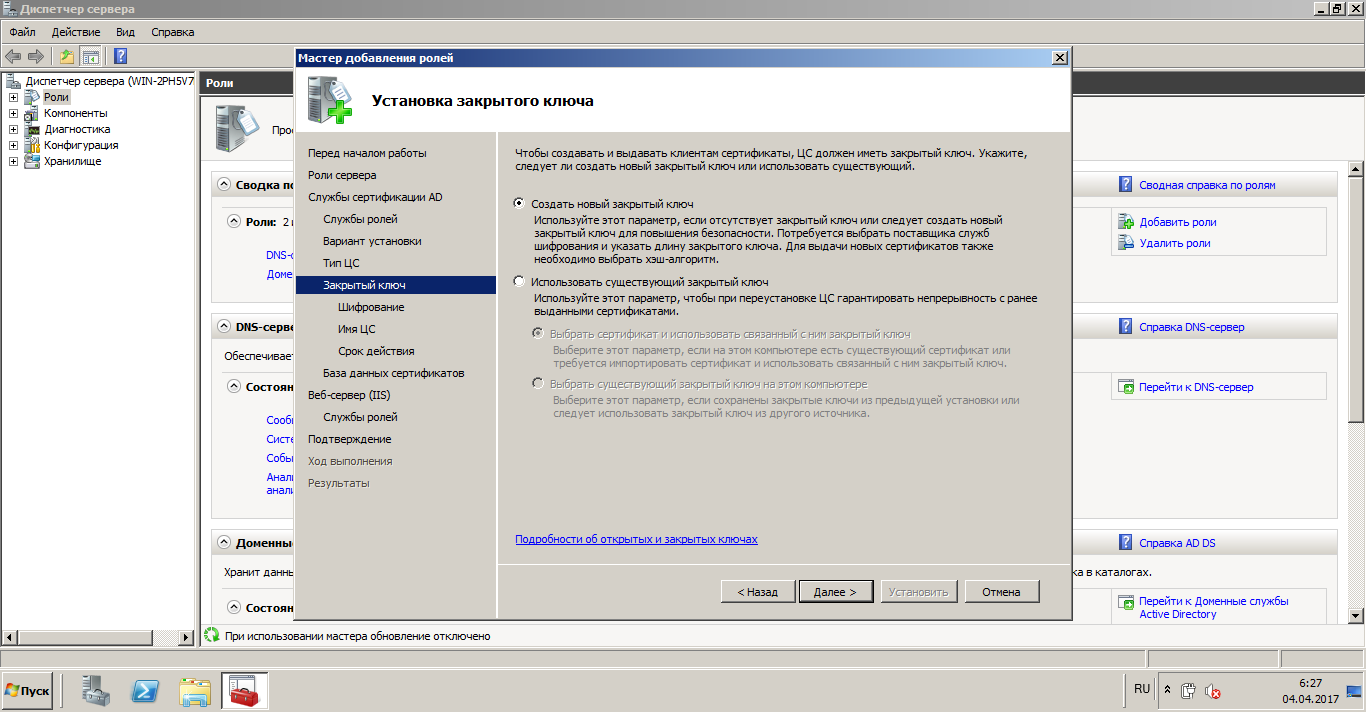
\includegraphics[width=1\textwidth]{7}
    \caption{Архитектура DPDK}
    \label{img:7}
\end{figure} 

\clearpage

DPDK дает возможность:
\begin{itemize}
\item принимать и отправлять пакеты с использованием наименьшего количества циклов ЦП (обычно не более 80 циклов);
\item разрабатывать алгоритмы быстрой записи пакетов (наподобие tcpdump);
\item запускать быстрые стеки сторонних разработчиков.
\end{itemize}

Производительность некоторых функций обработки пакетов составляет миллионы кадров в секунду при использовании 64-байтовых пакетов с сетевыми платами PCIe\*.\par

DPDK это OpenSource проект Intel'a, на основе которого были построены целые конторы (6WIND) и для которого производители изредка предоставляют драйвера, например Mellanox. Естественно, коммерческая поддержка решений на его основе просто замечательная, её предоставляет довольно большое количество вендоров (6WIND, Aricent, ALTEN Calsoft Labs, Advantech, Brocade, Radisys,Tieto, Wind River, Lanner, Mobica).\par 
 
DPDK имеет наиболее широкий функционал, и лучше всего абстрагирует существующее железо, он создан достаточно гибким для достижения высокой, возможно максимальной, производительности.
DPDK не является набором сетевых протоколов и не реализует такие функции, как перенаправление уровня 3, IPsec, брандмауэр и т.д. \par 
